\chapter{Sets and Tables}

\textsc{Perspective}: Sets and tables are data aggregates that are
very useful for a number of common programming tasks.  Nevertheless,
few programming languages support these data types, with the notable
exceptions of Sail (Reiser 1976) and SETL (Dewar, Schonberg, and
Schwartz 1981). There are many reasons why these obviously useful data
types are not found in most programming languages, but perceived
implementation problems certainly rank high among them. If only for
this reason, their implementation in Icon is worth studying.

Historically, tables in Icon were inherited from SNOBOL4 and SL5. Sets
came later, as an extension to Icon, and were designed and implemented
as a class project. Although sets were a late addition to Icon, they
are simpler than tables.  Nonetheless, they present many of the same
implementation problems that tables do. Consequently, sets are
considered here first.

Sets and the operations on them support the familiar mathematical
concepts of finite sets: membership, the insertion and deletion of
members, and the operations of union, intersection, and
difference. What is interesting about a set in Icon is that it can
contain members of any data type. This is certainly a case where
heterogeneity significantly increases the usefulness of a data
aggregate without adding to the difficulty of the implementation,
\textit{per se.}

The ability of a set to grow and shrink in size influences the
implementation significantly. Efficient access to members of a set,
which is needed for testing membership as well as the addition and
deletion of members, is an important consideration, since sets can be
arbitrarily large.


Tables have more structure than sets. Abstractly, a table is a set of
pairs that represents a many-to-one relationship-a function. In this
sense, the default value of a table provides an extension of the
partial function represented by the entry and assigned value pairs to
a complete function over all possible entry values. Programmers,
however, tend to view tables in a more restricted way, using them to
tabulate the attributes of a set of values of interest. In fact,
before sets were added to Icon, tables were often used to simulate
sets by associating a specific assigned value with membership.

\section[7.1 Sets]{7.1 Sets}
\subsection[7.1.1 Data Organization for Sets]{7.1.1 Data Organization for Sets}

Hash lookup and linked lists are used to provide an efficient way of
locating set members. For every set there is a set-header block that
contains a word for the number of members in the set and slots that
serve as heads for (possibly empty) linked lists of set-element
blocks. The number of slots is an implementation parameter. There are
thirty-seven slots in table-header blocks on computers with large
address spaces but only thirteen slots on computers with small address
spaces.

The structure for an empty set, produced by

%-% \ \ \ s := set([])
\iconline{
\>s := set([])\\
}

\noindent is

%--%\ \  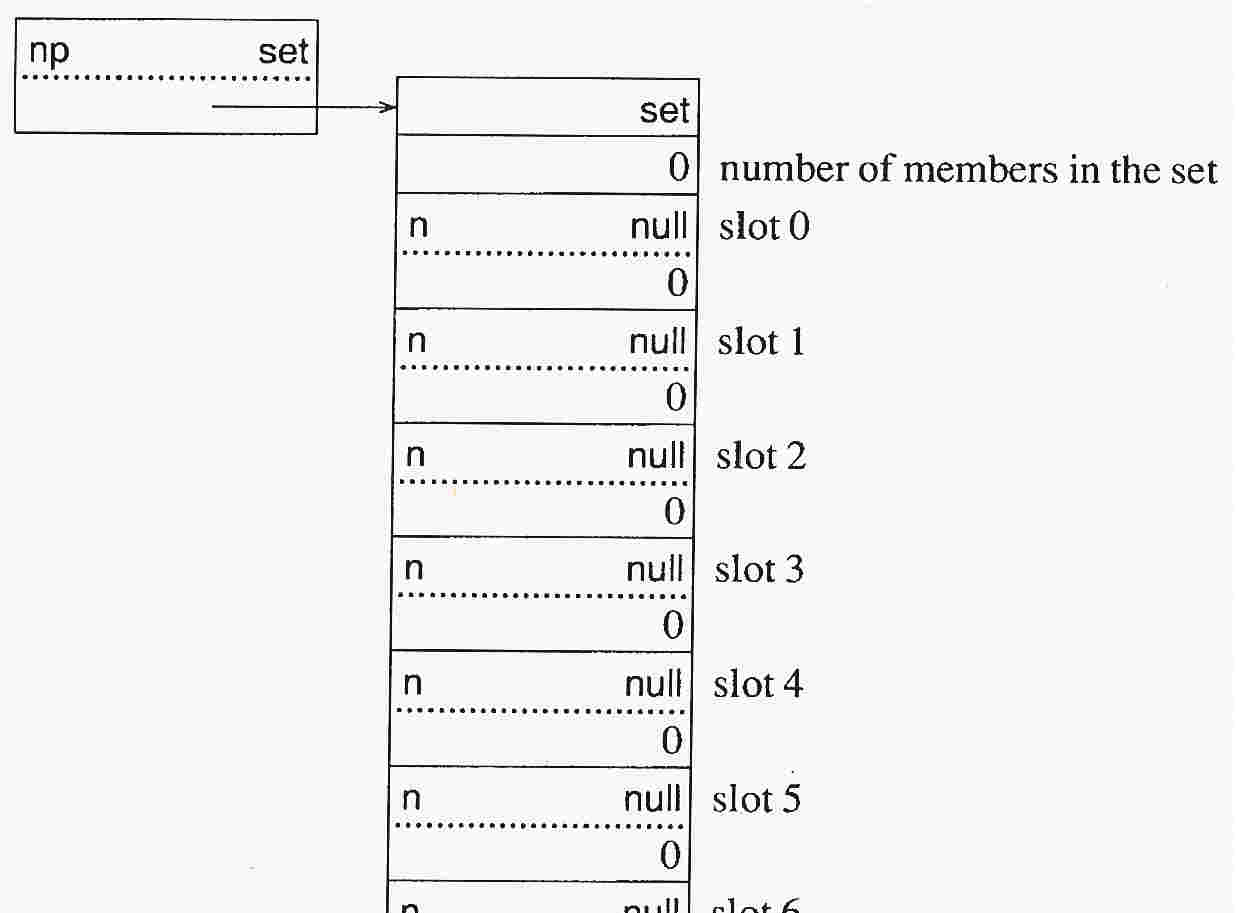
\includegraphics[width=4.1681in,height=3.0484in]{ib-img/ib-img034.jpg} 
\begin{picture}(300,250)(0,-30)
\put(120,0){\dvbox{null}{n}{0}}
\put(120,0){\trboxlabel{slot 4}}
\put(120,32){\dvbox{null}{n}{0}}
\put(120,32){\trboxlabel{slot 3}}
\put(120,64){\dvbox{null}{n}{0}}
\put(120,64){\trboxlabel{slot 2}}
\put(120,96){\dvbox{null}{n}{0}}
\put(120,96){\trboxlabel{slot 1}}
\put(120,128){\dvbox{null}{n}{0}}
\put(120,128){\trboxlabel{slot 0}}
\put(120,160){\blkbox{set}{0}}
\put(0,176){\dvptrbox{set}{np}{40}{}}
\put(120,0){\downetc}
\end{picture}

Each member of a set is contained in a separate set-element
block. When a value is looked up in a set (for example, to add a new
member), a hash number is computed from this value. The absolute value
of the remainder resulting from dividing the hash number by the number
of slots is used to select a slot.

Each set-element block contains a descriptor for its value, the
corresponding hash number, and a pointer to the next set-element
block, if any, on the linked list. For example, the set-element block
for the integer 39 is:

%--%\ \ \ \ \ \  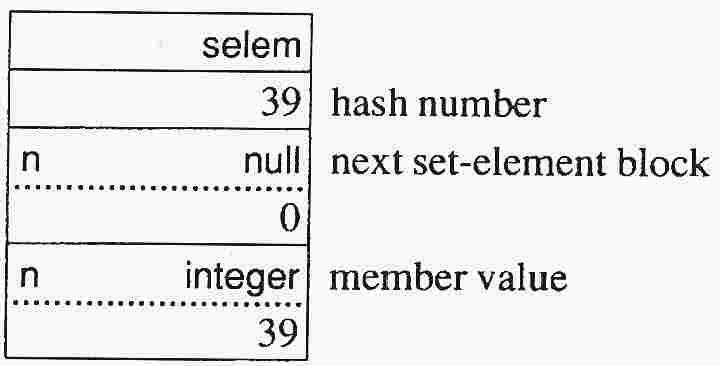
\includegraphics[width=2.4575in,height=1.2217in]{ib-img/ib-img035.jpg} 
\begin{picture}(300,90)
\put(120,0){\dvbox{integer}{n}{39}}
\put(120,0){\trboxlabel{member value}}
\put(120,32){\dvbox{null}{n}{0}}
\put(120,32){\trboxlabel{next set-element block}}
\put(120,64){\blkbox{selem}{39}}
\put(120,64){\trboxlabel{hash number}}
\end{picture}

As illustrated by this figure, the hash number for an integer is just
the value of the integer. This member goes in slot 2 on computers with
large address spaces, since its remainder on division by the number of
slots is two. Hash computation is discussed in detail in Sec. 7.3.

The structures for the set

%-% {\ttfamily\mdseries
%-% \ \ s := set([39,2])}
\iconline{
\ \ s := set([39,2])
}

\noindent are

%--%\ \  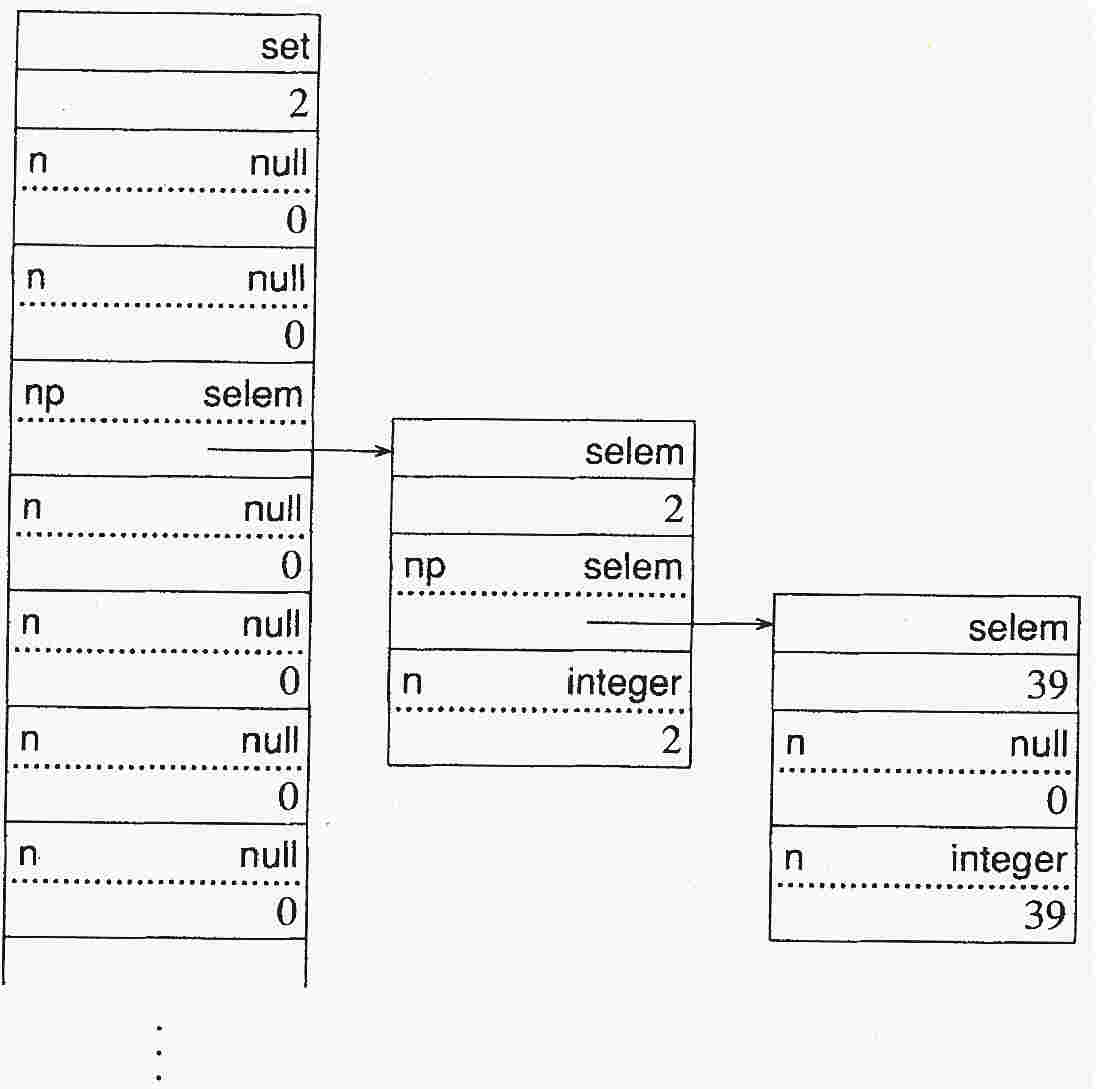
\includegraphics[width=3.7402in,height=3.6366in]{ib-img/ib-img036.jpg} 
\begin{picture}(300,290)(-40,-90)
\put(-4,0){\dvbox{null}{n}{0}}
\put(-4,32){\dvbox{null}{n}{0}}
\put(-4,64){\dvptrbox{selem}{n}{40}{}}
\put(-4,96){\dvbox{null}{n}{0}}
\put(-4,128){\dvbox{null}{n}{0}}
\put(-4,160){\blkbox{set}{2}}
\put(-4,0){\downetc}
\put(118,64){% 1st set member
\begin{picture}(100,96)(2,78)
\put(0,0){\dvbox{integer}{n}{2}}
\put(0,32){\dvptrbox{selem}{np}{40}{}}
\put(0,64){\blkbox{selem}{2}}
\end{picture}
}
\put(236,64){% 2nd set member
\begin{picture}(100,96)(0,124)
\put(0,0){\dvbox{integer}{n}{39}}
\put(0,32){\dvbox{null}{n}{0}}
\put(0,64){\blkbox{selem}{39}}
\end{picture}
}
\end{picture}

This example was chosen for illustration, since both 2 and 39 go in slot 2.

In searching the list, the hash number of the value being looked up is
compared with the hash numbers in the set-element blocks. If a match
is found, the value in the set-element block mayor may not be the same
as the value being looked up, since collisions in the hash computation
are unavoidable. Thus, if the hash numbers are the same, it is
necessary to determine whether or not their values are equivalent. The
comparison that is used is the same one that is used by the
source-language operation \texttt{x === y}.

To improve the performance of the lookup process, the set-element
blocks in each linked list are ordered by their hash numbers. When a
linked list of set-element blocks is examined, the search stops if a
hash number of an element on the list is greater than the hash number
of the value being looked up.

If the value is not found and the lookup is being performed to insert
a new member, a set-element block for the new member is created and
linked into the list at that point. For example,

%-% {\ttfamily\mdseries
%-% \ \ \ insert(s, -39)}
\iconline{
\>insert(s, -39)
}

\noindent inserts a set-element block for -39 at the head of the list
in slot 2, since its hash value is -39. The word in the set-header
block that contains the number of members is incremented to reflect
the insertion.

\subsection[7.1.2 Set Operations]{7.1.2 Set Operations}

The set operations of union, intersection, and difference all produce
new sets and do not modify their arguments.


In the case of union, a copy of the larger set is made first to
provide the basis for the union. This involves not only copying the
set-header block but also all of its set-element blocks. These are
linked together as in the original set, and no lookup is
required. After this copy is made, each member of the set for the
other argument is inserted in the copy, using the same technique that
is used in insert. The larger set is copied, since copying does not
require lookup and the possible comparison of values that insertion
does. The insertion of a member from the second set may take longer,
however, since the linked lists in the copy may be longer.

In the case of intersection, a copy of the smaller argument set is
made, omitting any of its members that are not in the larger set. As
with union, this strategy is designed to minimize the number of
lookups.

For the difference of two sets, a copy of the first argument set is
made, adding only elements that are not in the second argument. This
involves looking up all members in the first argument set in the
second argument set.

\section[7.2 Tables]{7.2 Tables}
\subsection[7.2.1 Data Organization for Tables]{7.2.1 Data Organization for Tables}

The implementation of tables is similar to the implementation of sets,
with a header block containing slots for elements ordered by hash
numbers. A table-header block contains an extra descriptor for the
default assigned value.

An empty table with the default assigned value 0 is produced by

%-% {\ttfamily\mdseries
%-% \ \ \ t := table(0)}
\iconline{
\>t := table(0)
}

The structure of the table-header block is

%--%\ \  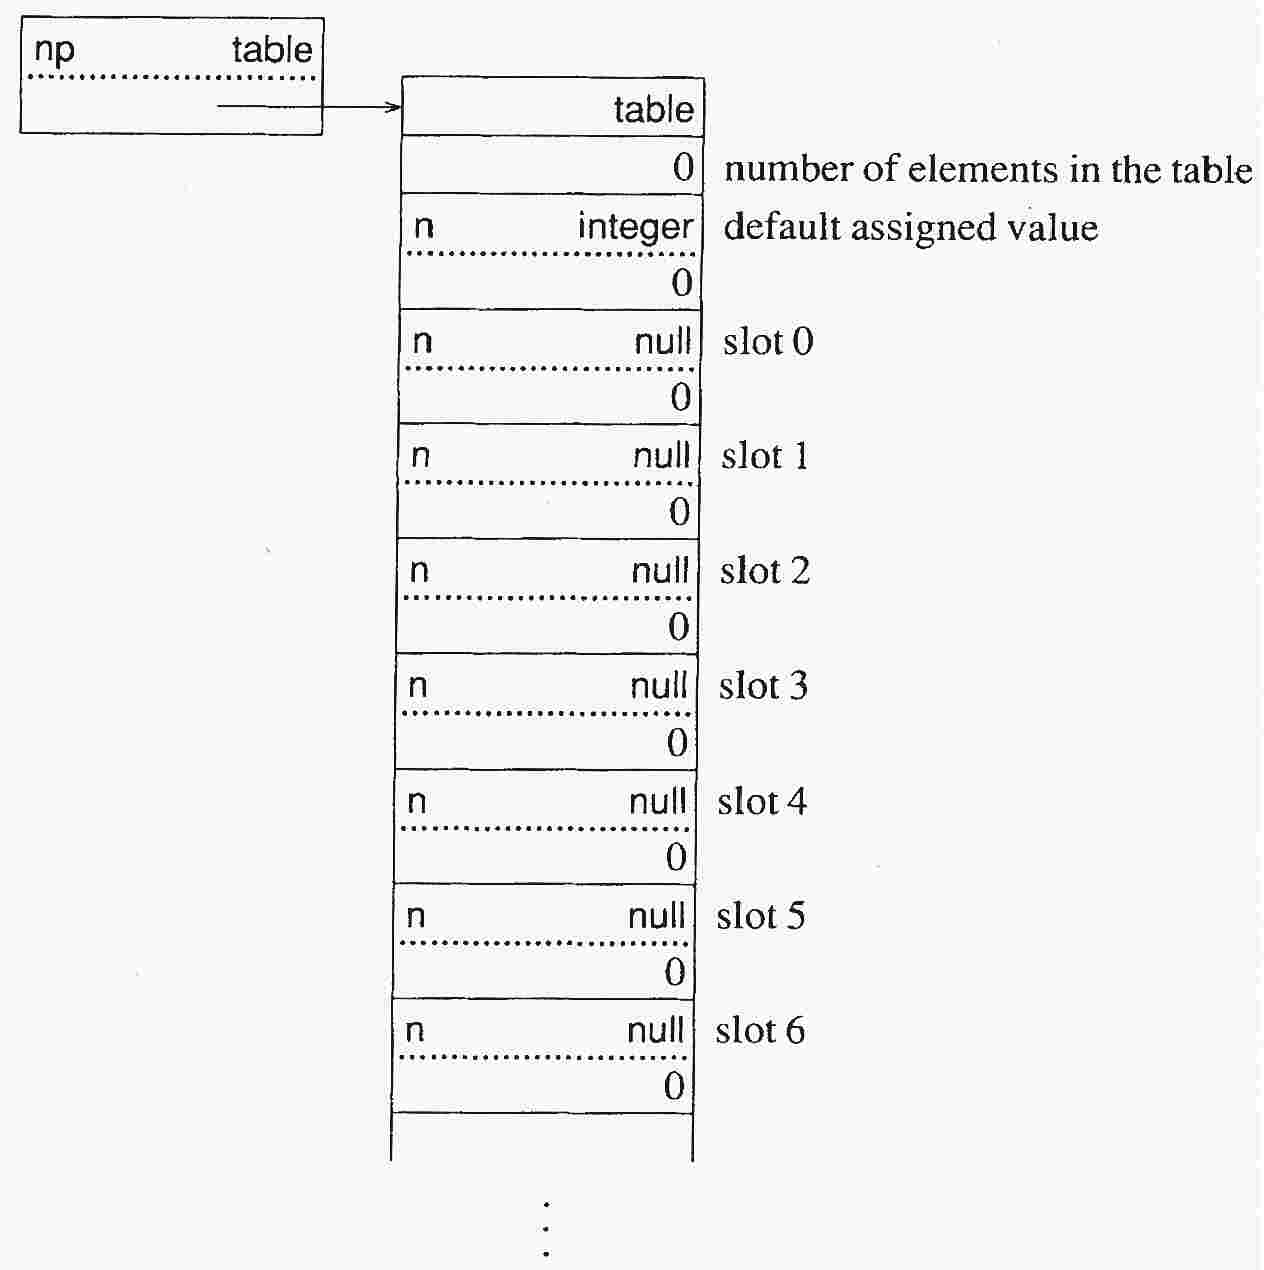
\includegraphics[width=4.2752in,height=4.2417in]{ib-img/ib-img037.jpg} 
\begin{picture}(300,280)(0,-30)
\put(120,0){\dvbox{null}{n}{0}}
\put(120,0){\trboxlabel{slot 4}}
\put(120,32){\dvbox{null}{n}{0}}
\put(120,32){\trboxlabel{slot 3}}
\put(120,64){\dvbox{null}{n}{0}}
\put(120,64){\trboxlabel{slot 2}}
\put(120,96){\dvbox{null}{n}{0}}
\put(120,96){\trboxlabel{slot 1}}
\put(120,128){\dvbox{null}{n}{0}}
\put(120,128){\trboxlabel{slot 0}}
\put(120,160){\dvbox{integer}{n}{0}}
\put(120,160){\trboxlabel{default assigned value}}
\put(120,192){\blkbox{table}{0}}
\put(120,192){\brboxlabel{number of elements in the table}}
\put(0,208){\dvptrbox{table}{np}{40}{}}
\put(120,0){\downetc}
\end{picture}

Table lookup is more complicated than set lookup, since table elements
contain both an entry value and an assigned value. Furthermore, table
elements can be referenced by variables. A new table element is
created as a byproduct of assignment to a table reference with an
entry value that is not in the table.

The result of evaluating an assignment expression such as

%-% {\ttfamily\mdseries
%-% \ \ \ t[39] := 1}
\iconline{
\>t[39] := 1
}

\noindent illustrates the structure of a table-element block:

%--%\ \  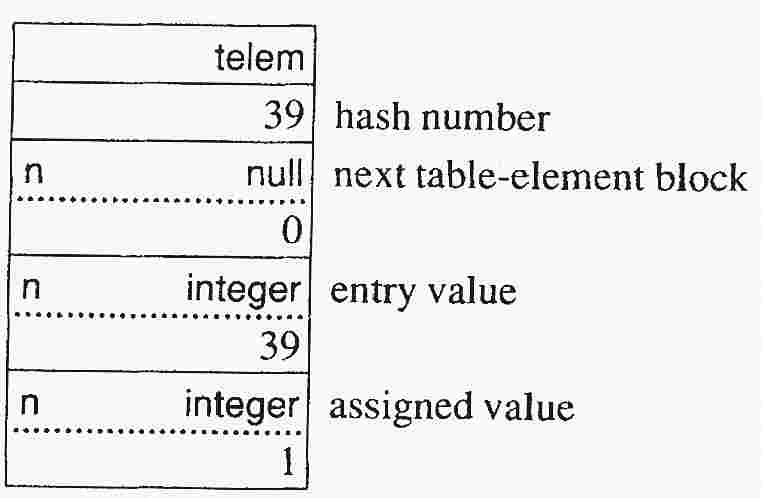
\includegraphics[width=2.5654in,height=1.6634in]{ib-img/ib-img038.jpg}
\begin{picture}(300,150)(50,-10)
\put(120,0){\dvbox{integer}{n}{1}}
\put(120,0){\trboxlabel{assigned value}}
\put(120,32){\dvbox{null}{n}{39}}
\put(120,32){\trboxlabel{entry value}}
\put(120,64){\dvbox{null}{n}{0}}
\put(120,64){\trboxlabel{next table-element block}}
\put(120,96){\blkbox{telem}{39}}
\put(120,96){\brboxlabel{hash number}}
\end{picture}

In the case of a table reference such as \texttt{t[x]}, the hash
number for the entry value x is used to select a slot, and the
corresponding list is searched for a table-element block that contains
the same entry value. As in the case of sets, comparison is first made
using hash numbers; values are compared only if their hash numbers are
the same.

If a table-element block with a matching entry value is found, a
variable that points to the corresponding assigned value is
produced. For example, if 39 is in t as illustrated previously,
\texttt{t[39]} produces

%--%\ \  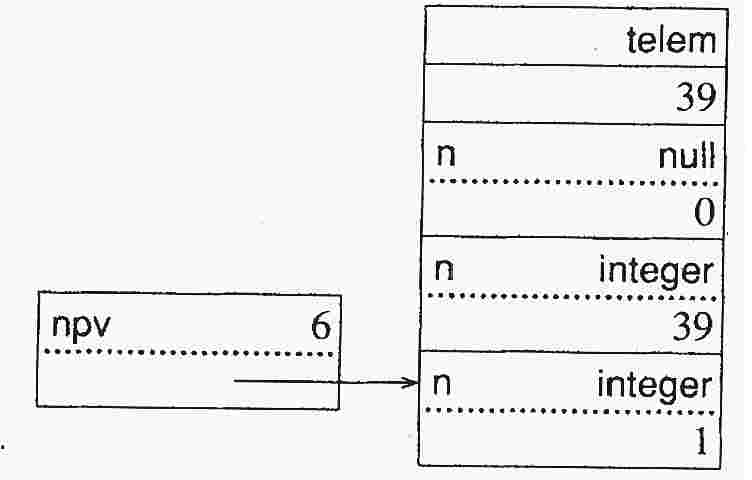
\includegraphics[width=2.5654in,height=1.602in]{ib-img/ib-img039.jpg} 
\begin{picture}(300,150)
\put(120,0){\dvbox{integer}{n}{1}}
\put(120,32){\dvbox{integer}{n}{39}}
\put(120,64){\dvbox{null}{n}{0}}
\put(120,96){\blkbox{telem}{39}}
\put(0,16){\dvptrbox{6}{npv}{40}{}}
\end{picture}

If this variable is dereferenced, as in

%-% {\ttfamily\mdseries
%-% \ \ \ write(t[39])}
\iconline{
\>write(t[39])
}

\noindent the value 1 is written. On the other hand, if an assignment
is made to this variable, as in

%-% {\ttfamily\mdseries
%-% \ \ \ t[39] +:= 1}
\iconline{
\>t[39] +:= 1
}

\noindent the assigned value in the table-element block is changed:

%--%\ \  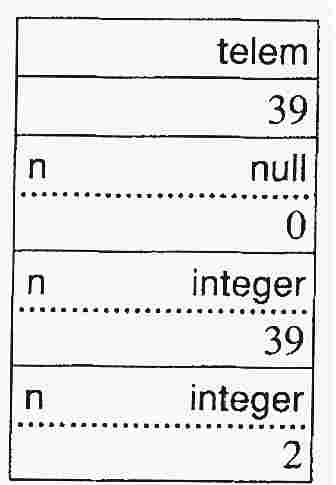
\includegraphics[width=1.1752in,height=1.6189in]{ib-img/ib-img040.jpg} 
\begin{picture}(300,150)(50,0)
\put(120,0){\dvbox{integer}{n}{2}}
\put(120,32){\dvbox{integer}{n}{39}}
\put(120,64){\dvbox{null}{n}{0}}
\put(120,96){\blkbox{telem}{39}}
\end{picture}

If a table element with a matching entry value is not found, the
situation is very similar to that in a subscripted string: the
operation to be performed depends on whether the table reference is
used in a dereferencing or assignment context. In a dereferencing
context, the default value for the table is produced, while in an
assignment context, a new element is added to the table.

The approach taken is similar to that for subscripted strings: a
trapped variable is created. As with substring trapped variables,
table-element trapped variables contain the information that is
necessary to carry out the required computation for either
dereferencing or assignment.

Suppose, for example, that the entry value \texttt{36} is not in the
table \texttt{t}. Then \texttt{t[36]} produces the following result:

%--%\ \  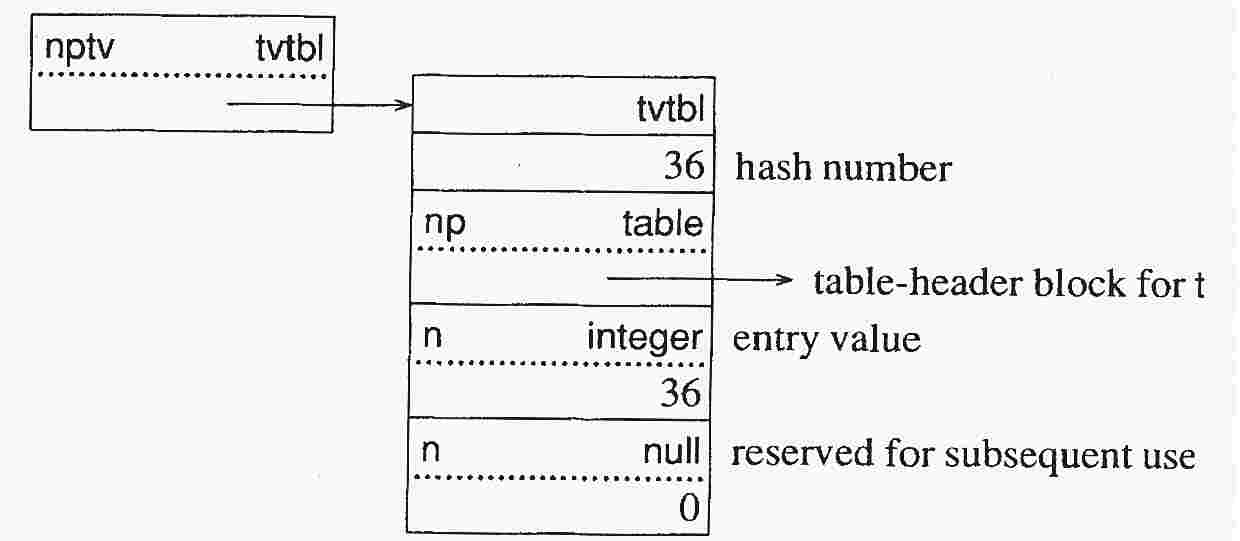
\includegraphics[width=4.1681in,height=1.8071in]{ib-img/ib-img041.jpg} 
\begin{picture}(300,150)
\put(120,0){\dvbox{null}{n}{0}}
\put(120,0){\trboxlabel{reserved for subsequent use}}
\put(120,32){\dvbox{integer}{n}{36}}
\put(120,32){\trboxlabel{entry value}}
\put(120,64){\dvptrbox{table}{np}{40}{table header block for t}}
\put(120,96){\blkbox{tvtbl}{36}}
\put(120,96){\brboxlabel{hash number}}
\put(0,112){\dvptrbox{tvtbl}{nptv}{40}{}}
\end{picture}

Note that the size of a table-element trapped-variable block is the
same as the size of a table-element block. The last descriptor in the
table-element trapped-variable block is reserved for subsequent use,
as described below.

If this trapped variable is dereferenced, as in

%-% {\ttfamily\mdseries
%-% \ \ \ write(t[36])}
\iconline{
\>write(t[36])
}

\noindent the default assigned value, 0, which is in the table-header
block for \texttt{t}, is produced. Unfortunately, the situation is not
always this simple. It is possible for elements to be inserted in a
table between the time the table-element trapped-variable block is
created and the time it is dereferenced. An example is

%-% {\ttfamily\mdseries
%-% \ \ \ write(t[36] , t[36] := 2)}
\iconline{
\>write(t[36] , t[36] := 2)
}

Since functions do not dereference their arguments until all the
arguments have been evaluated, the result of dereferencing the first
argument of write should be 2, not 0. In order to handle such cases,
when a table-element trapped variable is dereferenced, its linked list
in the table must be searched again to determine whether to return the
assigned value of a newly inserted element or to return the default
value.

If an assignment is made to the table reference, as in

%-% {\ttfamily\mdseries
%-% \ \ \ t[36] +:= 1}
\iconline{
\>t[36] +:= 1
}

\noindent the table-element trapped-variable block is converted to a
table-element block with the assigned value stored in the reserved
descriptor of the table-element trapped-variable block. The
table-element block is then linked in the appropriate place. Note that
the structures of table-element blocks and table-element
trapped-variable blocks are the same, allowing this conversion without
allocating a new table-element block.

It then is necessary to search the linked list for its slot again to
determine the place to insert the table-element block. As in the case
of dereferencing, elements may have been inserted in the table between
the time the table-element trapped variable was created and the time a
value is assigned to it. Normally, no matching entry is found, and the
table-element trapped-variable block, transformed into a table-element
block, is inserted with the new assigned value.  If a matching entry
is found, its assigned value is simply changed, and the block is
discarded.

Note that reference to a value that is not in a table requires only
one computation of its hash value, but two lookups are required in the
linked list of table-element blocks for its slot.


\section[7.3 Hashing Functions]{7.3 Hashing Functions}

Ideally, a hash computation should produce a different result for
every different value to which it is applied, and the distribution of
the remainder on division by the number of slots should be
uniform. Even approaching this ideal requires an impractical amount of
computation and space. In practice, it is desirable to have a fast
computation that produces few collisions.

The subject of hash computation has been studied extensively and there
is a substantial body of knowledge concerning useful techniques (Knuth
1973, pp. 506-549). For example, it is known that the number of slots
should be a prime that is not close to a power of two. This
consideration motivated the choices of 37 and 13 for computers with
large and small address spaces, respectively. In general, there is a
trade-off between faster lookup, on the average, and more storage
overhead.

In most situations in which hashing techniques are used, all the
values for which hash computations are performed are strings. In Icon,
however, any kind of value can be the member of a set or the entry
value in a table. The hash computation must, therefore, apply to any
type of value. The support routine for computing hash numbers is

%-% {\ttfamily
%-% uword hash(dp)
%-% 
%-% dptr dp;
%-% 
%-% \ \ \ \{
%-% 
%-% \ \ \ register char *s;
%-% 
%-% \ \ \ register uword i;
%-% 
%-% \ \ \ register word j, n;
%-% 
%-% \ \ \ register unsigned int *bitarr;
%-% 
%-% \ \ \ double r;
%-% 
%-% \ \ \ if (Qual(*dp)) \{
%-% 
%-% \ \ \ hashstring:
%-% 
%-% \ \ \ \ \ \ /*
%-% 
%-% \ \ \ \ \ \ \ * Compute the hash value for the string based on a scaled 
%-% 
%-% \ \ \ \ \ \ \ * \ sum of its first ten characters, plus its length.
%-% 
%-% \ \ \ \ \ \ \ */
%-% 
%-% \ \ \ \ \ \ i = 0;
%-% 
%-% \ \ \ \ \ \ s = StrLoc(*dp);
%-% 
%-% \ \ \ \ \ \ j = n = StrLen(*dp);
%-% 
%-% \ \ \ \ \ \ if (j {\textgreater} 10)\ \ /* limit scan to first ten characters */
%-% 
%-% \ \ \ \ \ \ \ \ \ j = 10;
%-% 
%-% \ \ \ \ \ \ while (j-{}- {\textgreater} 0) \{
%-% 
%-% \ \ \ \ \ \ \ \ \ i += *s++ \& 0xFF;\ \ /* add unsigned version of char */
%-% 
%-% \ \ \ \ \ \ \ \ \ i *= 37;\ \ \ \ /* scale by a nice prime number */
%-% 
%-% \ \ \ \ \ \ \ \ \ \}
%-% 
%-% \ \ \ \ \ \ i += n;\ \ \ \ \ \ /* add (untruncated) string length */
%-% 
%-% \ \ \ \ \ \ \}
%-% 
%-% \ \ \ else \{
%-% 
%-% \ \ \ \ \ \ switch (Type(*dp)) \{
%-% 
%-% \ \ \ \ \ \ \ \ \ /*
%-% 
%-% \ \ \ \ \ \ \ \ \ \ * The hash value of an integer is itself times eight 
%-% 
%-% \ \ \ \ \ \ \ \ \ \ * \ times the golden ratio. \ We do this calculation in 
%-% 
%-% \ \ \ \ \ \ \ \ \ \ * \ fixed point. \ We don't just use the integer itself, 
%-% 
%-% \ \ \ \ \ \ \ \ \ \ * \ for that would give bad results with sets having
%-% 
%-% \ \ \ \ \ \ \ \ \ \ * \ entries that are multiples of a power of two.
%-% 
%-% \ \ \ \ \ \ \ \ \ \ */
%-% 
%-% \ \ \ \ \ \ \ \ \ case T\_Integer:
%-% 
%-% \ \ \ \ \ \ \ \ \ \ \ \ i = (13255 * (uword)IntVal(*dp)) {\textgreater}{\textgreater} 10;
%-% 
%-% \ \ \ \ \ \ \ \ \ \ \ \ break;
%-% 
%-% \ \ \ \ \ \ \ \ \ /*
%-% 
%-% \ \ \ \ \ \ \ \ \ \ * The hash value of a bignum is based on its length and 
%-% 
%-% \ \ \ \ \ \ \ \ \ \ * \ its most and least significant digits.
%-% 
%-% \ \ \ \ \ \ \ \ \ \ */
%-% 
%-% \ \  case T\_Lrgint:
%-% 
%-% \ \  \ \ \ \{
%-% 
%-% \ \  \ \ \ struct b\_bignum *b = \&BlkLoc(*dp)-{\textgreater}bignumblk;
%-% 
%-% \ \  \ \ \ i = ((b-{\textgreater}lsd - b-{\textgreater}msd) {\textless}{\textless} 16) \^{}
%-% 
%-% \ \ \ \ (b-{\textgreater}digits[b-{\textgreater}msd] {\textless}{\textless} 8) \^{}
%-% b-{\textgreater}digits[b-{\textgreater}lsd];
%-% 
%-% \ \  \ \ \ \}
%-% 
%-% \ \  \ \ \ break;
%-% 
%-% \ \ \ \ \ \ \ \ \ /*
%-% 
%-% \ \ \ \ \ \ \ \ \ \ * The hash value of a real number is itself times a 
%-% 
%-% \ \ \ \ \ \ \ \ \ \ * \ constant, converted to an unsigned integer. \ The 
%-% 
%-% \ \ \ \ \ \ \ \ \ \ * \ intent is to scramble the bits well, in the case of 
%-% 
%-% \ \ \ \ \ \ \ \ \ \ * \ integral values, and to scale up fractional values 
%-% 
%-% \ \ \ \ \ \ \ \ \ \ * \ so they don't all land in the same bin. The constant
%-% 
%-% \ \ \ \ \ \ \ \ \ \ * \ below is 32749 / 29, the quotient of two primes,
%-% 
%-% \ \ \ \ \ \ \ \ \ \ * \ and was observed to work well in empirical testing.
%-% 
%-% \ \ \ \ \ \ \ \ \ \ */
%-% 
%-% \ \ \ \ \ \ \ \ \ case T\_Real:
%-% 
%-% \ \ \ \ \ \ \ \ \ \ \ \ GetReal(dp,r);
%-% 
%-% \ \ \ \ \ \ \ \ \ \ \ \ i = r * 1129.27586206896558;
%-% 
%-% \ \ \ \ \ \ \ \ \ \ \ \ break;
%-% 
%-% \ \ \ \ \ \ \ \ \ /*
%-% 
%-% \ \ \ \ \ \ \ \ \ \ * The hash value of a cset is based on a convoluted 
%-% 
%-% \ \ \ \ \ \ \ \ \ \ * \ combination of all its bits.
%-% 
%-% \ \ \ \ \ \ \ \ \ \ */
%-% 
%-% \ \ \ \ \ \ \ \ \ case T\_Cset:
%-% 
%-% \ \ \ \ \ \ \ \ \ \ \ \ i = 0;
%-% 
%-% \ \ \ \ \ \ \ \ \ \ \ \ bitarr = BlkLoc(*dp)-{\textgreater}cset.bits + CsetSize - 1;
%-% 
%-% \ \ \ \ \ \ \ \ \ \ \ \ for (j = 0; j {\textless} CsetSize; j++) \{
%-% 
%-% \ \ \ \ \ \ \ \ \ \ \ \ \ \ \ i += *bitarr-{}-;
%-% 
%-% \ \ \ \ \ \ \ \ \ \ \ \ \ \ \ i *= 37;\ \ \ \ \ \ /* better distribution */
%-% 
%-% \ \ \ \ \ \ \ \ \ \ \ \ \ \ \ \}
%-% 
%-% \ \ \ \ \ \ \ \ \ \ \ \ i \%= 1048583;\ \ \ \ /* scramble the bits */
%-% 
%-% \ \ \ \ \ \ \ \ \ \ \ \ break;
%-% 
%-% \ \ \ \ \ \ \ \ \ /*
%-% 
%-% \ \ \ \ \ \ \ \ \ \ * The hash value of a list, set, table, or record is 
%-% 
%-% \ \ \ \ \ \ \ \ \ \ * \ its id, hashed like an integer.
%-% 
%-% \ \ \ \ \ \ \ \ \ \ */
%-% 
%-% \ \ \ \ \ \ \ \ \ case T\_List:
%-% 
%-% \ \ \ \ \ \ \ \ \ \ \ \ i = (13255 * BlkLoc(*dp)-{\textgreater}list.id) {\textgreater}{\textgreater} 10;
%-% 
%-% \ \ \ \ \ \ \ \ \ \ \ \ break;
%-% 
%-% \ \ \ \ \ \ \ \ \ case T\_Set:
%-% 
%-% \ \ \ \ \ \ \ \ \ \ \ \ i = (13255 * BlkLoc(*dp)-{\textgreater}set.id) {\textgreater}{\textgreater} 10;
%-% 
%-% \ \ \ \ \ \ \ \ \ \ \ \ break;
%-% 
%-% \ \ \ \ \ \ \ \ \ case T\_Table:
%-% 
%-% \ \ \ \ \ \ \ \ \ \ \ \ i = (13255 * BlkLoc(*dp)-{\textgreater}table.id) {\textgreater}{\textgreater} 10;
%-% 
%-% \ \ \ \ \ \ \ \ \ \ \ \ break;
%-% 
%-% \ \ \ \ \ \ \ \ \ case T\_Record:
%-% 
%-% \ \ \ \ \ \ \ \ \ \ \ \ i = (13255 * BlkLoc(*dp)-{\textgreater}record.id) {\textgreater}{\textgreater} 10;
%-% 
%-% \ \ \ \ \ \ \ \ \ \ \ \ break;
%-% 
%-% \ \  case T\_Proc:
%-% 
%-% \ \  \ \ \ dp = \&(BlkLoc(*dp)-{\textgreater}proc.pname);
%-% 
%-% \ \  \ \ \ goto hashstring;
%-% 
%-% \ \ \ \ \ \ \ \ \ default:
%-% 
%-% \ \ \ \ \ \ \ \ \ \ \ \ /*
%-% 
%-% \ \ \ \ \ \ \ \ \ \ \ \ \ * For other types, use the type code as the hash
%-% 
%-% \ \ \ \ \ \ \ \ \ \ \ \ \ * \ value.
%-% 
%-% \ \ \ \ \ \ \ \ \ \ \ \ \ */
%-% 
%-% \ \ \ \ \ \ \ \ \ \ \ \ i = Type(*dp);
%-% 
%-% \ \ \ \ \ \ \ \ \ \ \ \ break;
%-% 
%-% \ \ \ \ \ \ \ \ \ \}
%-% 
%-% \ \ \ \ \ \ \}
%-% 
%-% \ \ \ return i;
%-% 
%-% \ \ \ \}
%-% }
\iconcode{
uword hash(dp)\\
dptr dp;\\
\>\{\\
\>register char *s;\\
\>register uword i;\\
\>register word j, n;\\
\>register unsigned int *bitarr;\\
\>double r;\\
\>if (Qual(*dp)) \{\\
\>hashstring:\\
\>\>/*\\
\>\>\ * Compute the hash value for the string based on a scaled \\
\>\>\ * \ sum of its first ten characters, plus its length.\\
\>\>\ */\\
\>\>i = 0;\\
\>\>s = StrLoc(*dp);\\
\>\>j = n = StrLen(*dp);\\
\>\>if (j > 10)\ \ /* limit scan to first ten characters */\\
\>\>\>j = 10;\\
\>\>while (j-{}- > 0) \{\\
\>\>\>i += *s++ \& 0xFF;\ \ /* add unsigned version of char */\\
\>\>\>i *= 37;\ \ \ \ /* scale by a nice prime number */\\
\>\>\>\}\\
\>\>i += n;\ \ \ \ \ \ /* add (untruncated) string length */\\
\>\>\}\\
\>else \{\\
\>\>switch (Type(*dp)) \{\\
\>\>\>/*\\
\>\>\>\ * The hash value of an integer is itself times eight \\
\>\>\>\ * \ times the golden ratio. \ We do this calculation in \\
\>\>\>\ * \ fixed point. \ We don't just use the integer itself, \\
\>\>\>\ * \ for that would give bad results with sets having\\
\>\>\>\ * \ entries that are multiples of a power of two.\\
\>\>\>\ */\\
\>\>\>case T\_Integer:\\
\>\>\>\>i = (13255 * (uword)IntVal(*dp)) >> 10;\\
\>\>\>\>break;\\
\>\>\>/*\\
\>\>\>\ * The hash value of a bignum is based on its length and \\
\>\>\>\ * \ its most and least significant digits.\\
\>\>\>\ */\\
\>\>case T\_Lrgint:\\
\>\>\>\{\\
\>\>\>struct b\_bignum *b = \&BlkLoc(*dp)->bignumblk;\\
\>\>\>i = ((b->lsd - b->msd) <{}< 16) \^{}\\
\>\>\>\>(b->digits[b->msd] <{}< 8) \^{}\\
\>\>\>\>b->digits[b->lsd];\\
\>\>\>\}\\
\>\>\>break;\\
\>\>\>/*\\
\>\>\>\ * The hash value of a real number is itself times a \\
\>\>\>\ * \ constant, converted to an unsigned integer. \ The \\
\>\>\>\ * \ intent is to scramble the bits well, in the case of \\
\>\>\>\ * \ integral values, and to scale up fractional values \\
\>\>\>\ * \ so they don't all land in the same bin. The constant\\
\>\>\>\ * \ below is 32749 / 29, the quotient of two primes,\\
\>\>\>\ * \ and was observed to work well in empirical testing.\\
\>\>\>\ */\\
\>\>\>case T\_Real:\\
\>\>\>\>GetReal(dp,r);\\
\>\>\>\>i = r * 1129.27586206896558;\\
\>\>\>\>break;\\
\>\>\>/*\\
\>\>\>\ * The hash value of a cset is based on a convoluted \\
\>\>\>\ * \ combination of all its bits.\\
\>\>\>\ */\\
\>\>\>case T\_Cset:\\
\>\>\>\>i = 0;\\
\>\>\>\>bitarr = BlkLoc(*dp)->cset.bits + CsetSize - 1;\\
\>\>\>\>for (j = 0; j < CsetSize; j++) \{\\
\>\>\>\>\>i += *bitarr-{}-;\\
\>\>\>\>\>i *= 37;\ \ \ \ \ \ /* better distribution */\\
\>\>\>\>\>\}\\
\>\>\>\>i \%= 1048583;\ \ \ \ /* scramble the bits */\\
\>\>\>\>break;\\
\>\>\>/*\\
\>\>\>\ * The hash value of a list, set, table, or record is \\
\>\>\>\ * \ its id, hashed like an integer.\\
\>\>\>\ */\\
\>\>\>case T\_List:\\
\>\>\>\>i = (13255 * BlkLoc(*dp)->list.id) >> 10;\\
\>\>\>\>break;\\
\>\>\>case T\_Set:\\
\>\>\>\>i = (13255 * BlkLoc(*dp)->set.id) >> 10;\\
\>\>\>\>break;\\
\>\>\>case T\_Table:\\
\>\>\>\>i = (13255 * BlkLoc(*dp)->table.id) >> 10;\\
\>\>\>\>break;\\
\>\>\>case T\_Record:\\
\>\>\>\>i = (13255 * BlkLoc(*dp)->record.id) >> 10;\\
\>\>\>\>break;\\
\ \  case T\_Proc:\\
\ \  \ \ \ dp = \&(BlkLoc(*dp)->proc.pname);\\
\ \  \ \ \ goto hashstring;\\
\>\>\>default:\\
\>\>\>\>/*\\
\>\>\>\>\ * For other types, use the type code as the hash\\
\>\>\>\>\ * \ value.\\
\>\>\>\>\ */\\
\>\>\>\>i = Type(*dp);\\
\>\>\>\>break;\\
\>\>\>\}\\
\>\>\}\\
\>return i;\\
\>\}
}

To hash a string, its characters are added together as integers. At
most ten characters are used, since strings can be very long and
adding many characters does not improve the hashing sufficiently to
justify the time spent in the computation. The maximum of ten is,
however, \textit{ad hoc}. To provide a measure of discrimination
between strings with the same initial substring, the length of the
string is added to the sum of the characters. This technique for
hashing strings is not sophisticated, and others that produce better
hashing results are known. However, the computation is simple, easy to
write in C, and works well in practice.

For a numeric type, the hash value is derived from the number. In the
case of a cset, the words containing the bits for the cset are
combined using the exclusive-or operation.

The remaining data types pose an interesting problem. Hash computation
must be based on attributes of a value that are invariant with
time. Some types, such as files, have such attributes. On the other
hand, there is no time-invariant attribute that distinguishes one list
from another. The size of a list may change, the elements in it may
change, and even its location in memory may change as the result of
garbage collection. For a list, its only time-invariant attribute is
its type.

This presents a dilemma--the type of such a value can be used as its
hash number, but if that is done, all values of that type are in the
same slot and have the same hash number. Lookup for these values
degenerates to a linear search.  The alternative is to add some
time-invariant attribute, such as a serial number, to these
values. Icon does this, at the cost of increasing the size of every
such value.

\textsc{Retrospective}: Few programming languages support sets or
tables with Icon's generality. The implementation of sets and tables
provides a clear focus on the generality of descriptors and the
uniformity with which different kinds of data are treated in Icon.

Since sets and tables may be very large, efficient lookup is an
important concern. The hashing and chaining technique used is only one
of many possibilities. However, there must be a mechanism for
determining the equivalence of values independent of the structure in
which they are stored.

The fact that elements in tables are accessed by subscripting
expressions introduces several complexities. In particular, the fact
that the contents of the table that is subscripted may change between
the time the subscripting expression is evaluated and the time it is
dereferenced or assigned to introduces the necessity of two lookups
for every table reference.

Hashing a variety of different types of data raises interesting
issues. The hashing techniques used by Icon are not sophisticated and
there is considerable room for improvement. The trade-offs involved
are difficult to evaluate, however.

\bigskip

\noindent\textbf{EXERCISES}

\liststyleLvii
\begin{enumerate}
\item \begin{enumerate}

\item Contrast sets and csets with respect to their implementation,
their usefulness in programming, and the efficiency of operations on
them.

\item Give an example of a situation in which the heterogeneity of
sets is useful in programming.

\item How much space does an empty set occupy?

\item Diagram the structures resulting from the evaluation of the
following expressions:\newline
 t := table()\newline
 t[t] := t

\item There are many sophisticated data structures that are designed
to ensure efficient lookup in data aggregates like sets and tables
(Gonnet 1984). Consider the importance of speed of lookup in sets and
tables in Icon and the advantages that these more sophisticated data
structures might supply.

\item Some of the more sophisticated data structures mentioned in the
preceding exercise have been tried experimentally in Icon and either
have introduced unexpected implementation problems or have not
provided a significant improvement in performance. What are possible
reasons for these disappointing results?

\item Icon goes to a lot of trouble to avoid adding table-element
blocks to a table unless an assignment is made to them.  Suppose a
table-element block were simply added when a reference was made to an
entry value that is not in the table.
\end{enumerate}
\end{enumerate}
\liststyleLviii
\begin{itemize}
\item How would this simplify the implementation?

\item What positive and negative consequences could this change have
on the running speed and space required during program execution?

\item Give examples of types of programs for which the change would
have positive and negative effects on performance, respectively.

\item Would this change be transparent to the Icon programmer, not
counting possible time and space differences?
\end{itemize}
\liststyleLix
\begin{enumerate}
\item \begin{enumerate}

\item There is space in a table-element trapped-variable block to put
the default value for the table. Why is this not done?

\item 
What is the consequence of evaluating the following expressions?
\end{enumerate}
\end{enumerate}
%-% {\ttfamily\mdseries
%-% \ \ \ t := table(0)}
%-% 
%-% {\ttfamily\mdseries
%-% \ \ \ t[37] := 2}
%-% 
%-% {\ttfamily\mdseries
%-% \ \ \ write(t[37], t := table(1))}
\iconcode{
\>t := table(0)\\
\>t[37] := 2\\
\>write(t[37], t := table(1))
}

What would happen if the last line given previously were

%-% {\ttfamily\mdseries
%-% \ \ \ write(t[37],t := list(100,3))}
\iconline{
\>write(t[37],t := list(100,3))
}

or

%-% {\ttfamily\mdseries
%-% \ \ \ write(t[37], t := {\textquotedbl}hello{\textquotedbl})}
\iconline{
\>write(t[37], t := "hello")
}

\liststyleLx
\begin{enumerate}
\item \begin{enumerate}

\item Give examples of different strings that have the same hash numbers.

\item Design a method for hashing strings that produces a better
distribution than the the current one.

\item What attribute of a table is time-invariant?

\item What kinds of symptoms might result from a hashing computation
 based on an attribute of a value that is not time-invariant?

\end{enumerate}
\end{enumerate}
